
\documentclass[11pt,twoside]{article}
\usepackage{etex}

\raggedbottom

%geometry (sets margin) and other useful packages
\usepackage{geometry}
\geometry{top=1in, left=1in,right=1in,bottom=1in}
 \usepackage{graphicx,booktabs,calc}
 
\usepackage{listings}


% Marginpar width
%Marginpar width
\newcommand{\pts}[1]{\marginpar{ \small\hspace{0pt} \textit{[#1]} } } 
\setlength{\marginparwidth}{.5in}
%\reversemarginpar
%\setlength{\marginparsep}{.02in}

 
%\usepackage{cmbright}lstinputlisting
%\usepackage[T1]{pbsi}


\usepackage{chngcntr,mathtools}
%\counterwithin{figure}{section}
%\numberwithin{equation}{section}

%\usepackage{listings}

%AMS-TeX packages
\usepackage{amssymb,amsmath,amsthm} 
\usepackage{bm}
\usepackage[mathscr]{eucal}
\usepackage{colortbl}
\usepackage{color}


\usepackage{subfig,hyperref,enumerate,polynom,polynomial}
\usepackage{multirow,minitoc,fancybox,array,multicol}

\definecolor{slblue}{rgb}{0,.3,.62}
\hypersetup{
    colorlinks,%
    citecolor=blue,%
    filecolor=blue,%
    linkcolor=blue,
    urlcolor=slblue
}

%%%TIKZ
\usepackage{tikz}

\usepackage{pgfplots}
\pgfplotsset{compat=newest}

\usetikzlibrary{arrows,shapes,positioning}
\usetikzlibrary{decorations.markings}
\usetikzlibrary{shadows}
\usetikzlibrary{patterns}
%\usetikzlibrary{circuits.ee.IEC}
\usetikzlibrary{decorations.text}
% For Sagnac Picture
\usetikzlibrary{%
    decorations.pathreplacing,%
    decorations.pathmorphing%
}

\tikzstyle arrowstyle=[black,scale=2]
\tikzstyle directed=[postaction={decorate,decoration={markings,
    mark=at position .65 with {\arrow[arrowstyle]{stealth}}}}]
\tikzstyle reverse directed=[postaction={decorate,decoration={markings,
    mark=at position .65 with {\arrowreversed[arrowstyle]{stealth};}}}]
\tikzstyle dir=[postaction={decorate,decoration={markings,
    mark=at position .98 with {\arrow[arrowstyle]{latex}}}}]
\tikzstyle rev dir=[postaction={decorate,decoration={markings,
    mark=at position .98 with {\arrowreversed[arrowstyle]{latex};}}}]

\usepackage{ctable}

%
%Redefining sections as problems
%
\makeatletter
\newenvironment{exercise}{\@startsection 
	{section}
	{1}
	{-.2em}
	{-3.5ex plus -1ex minus -.2ex}
    	{1.3ex plus .2ex}
    	{\pagebreak[3]%forces pagebreak when space is small; use \eject for better results
	\large\bf\noindent{Part 1.\hspace{-1.5ex} }
	}
	}
	%{\vspace{1ex}\begin{center} \rule{0.3\linewidth}{.3pt}\end{center}}
	%\begin{center}\large\bf \ldots\ldots\ldots\end{center}}
\makeatother

%
%Fancy-header package to modify header/page numbering 
%
\usepackage{fancyhdr}
\pagestyle{fancy}
%\addtolength{\headwidth}{\marginparsep} %these change header-rule width
%\addtolength{\headwidth}{\marginparwidth}
%\fancyheadoffset{30pt}
%\fancyfootoffset{30pt}
\fancyhead[LO,RE]{\small Jimi Oke}
\fancyhead[RO,LE]{\small Page \thepage} 
\fancyfoot[RO,LE]{\small PS 1} 
\fancyfoot[LO,RE]{\small \scshape CEE 616} 
\cfoot{} 
\renewcommand{\headrulewidth}{0.1pt} 
\renewcommand{\footrulewidth}{0.1pt}
%\setlength\voffset{-0.25in}
%\setlength\textheight{648pt}


\usepackage{paralist}

\newcommand{\osn}{\oldstylenums}
\newcommand{\lt}{\left}
\newcommand{\rt}{\right}
\newcommand{\pt}{\phantom}
\newcommand{\tf}{\therefore}
\newcommand{\?}{\stackrel{?}{=}}
\newcommand{\fr}{\frac}
\newcommand{\dfr}{\dfrac}
\newcommand{\ul}{\underline}
\newcommand{\tn}{\tabularnewline}
\newcommand{\nl}{\newline}
\newcommand\relph[1]{\mathrel{\phantom{#1}}}
\newcommand{\cm}{\checkmark}
\newcommand{\ol}{\overline}
\newcommand{\rd}{\color{red}}
\newcommand{\bl}{\color{blue}}
\newcommand{\pl}{\color{purple}}
\newcommand{\og}{\color{orange!90!black}}
\newcommand{\gr}{\color{green!40!black}}
\newcommand{\nin}{\noindent}
\newcommand{\la}{\lambda}
\renewcommand{\th}{\theta}
\newcommand*\circled[1]{\tikz[baseline=(char.base)]{
            \node[shape=circle,draw,thick,inner sep=1pt] (char) {\small #1};}}

\newcommand{\bc}{\begin{compactenum}[\quad--]}
\newcommand{\ec}{\end{compactenum}}

\newcommand{\n}{\\[2mm]}
%% GREEK LETTERS
\newcommand{\al}{\alpha}
\newcommand{\gam}{\gamma}
\newcommand{\eps}{\epsilon}
\newcommand{\sig}{\sigma}

\newcommand{\p}{\partial}
\newcommand{\pd}[2]{\frac{\partial{#1}}{\partial{#2}}}
\newcommand{\dpd}[2]{\dfrac{\partial{#1}}{\partial{#2}}}
\newcommand{\pdd}[2]{\frac{\partial^2{#1}}{\partial{#2}^2}}
\newcommand{\mr}{\mathbb{R}}
\newcommand{\xs}{x^{*}}
\newenvironment{solution}
{\medskip\par\quad\quad\begin{minipage}[c]{.8\textwidth}}{\medskip\end{minipage}}

\newcommand{\nmfr}[3]{\Phi\left(\frac{{#1} - {#2}}{#3}\right)}
 
%%%%%%%%%%%%%%%%%%%%%%%%%%%%%%%%%%%%%%%%%%%%%%%%%%%
%%%%%%%%%%%%%%%%%%%%%%%%%%%%%%%%%%%%%%%%%%%%%%%%%%%

\begin{document}

\lstset{language=C++,
                basicstyle=\tiny\ttfamily,
                keywordstyle=\color{blue}\ttfamily,
                stringstyle=\color{red}\ttfamily,
                commentstyle=\color{gray}\ttfamily,
                morecomment=[l][\color{gray}]{\#}
}


\thispagestyle{empty}


\nin{\LARGE Problem Set 1 }\hfill{\bf Oke}

\medskip\hrule\medskip

\nin {\small CEE 616: Probabilistic Machine Learning
\hfill\textit{ 09.11.2025}}

\nin{\it \small Due  Thursday, September 25, 2025 at 11:59PM on Canvas}.\\

\nin The problems are worth a total of \textbf{85 points}.

\subsubsection*{Programming requirements}
It is recommended that you have a working installation of \href{https://jupyter.org/install.html}{JupyterLab}.
\href{https://colab.research.google.com/notebooks/intro.ipynb}{Google Colab} is also another viable notebook option.
However, notebooks are optional, and you can always choose to write your code in an editor (e.g. Sublime Text) and process your outputs accordingly. 

In Jupyter, you may use a Python, R or even MATLAB kernel.\footnote{In order to use the R kernel in Jupyter, you may have to install it, as well. Please follow the brief instructions here: \url{https://irkernel.github.io/installation/}. To install the MATLAB kernel, see \url{https://am111.readthedocs.io/en/latest/jmatlab_install.html}.}
Text can be formatted using Markdown (brief guide here: \url{https://learn.getgrav.org/content/markdown}).

Any Python packages you require must be installed locally to access them via the Jupyter kernel.
(Use \texttt{conda} or \texttt{pip}.)
 

\subsubsection*{Programming help}
I will provide some programming templates in Python/R in the coming days on Moodle, in order to ease some of the possible
issues that may arise as you begin scripting. We will also go over coding examples weekly.

\subsubsection*{Submission instructions}
There are two options for submission:
\begin{enumerate}
\item JupyterLab Notebook. Please name your notebook as follows: \\ \texttt{<lastname>-<firstname>-PS1.ipynb}
\item R/Python/MATLAB script \textit{and} PDF document with supporting responses.
  Your PDF should have complete responses to all the questions (including all the required plots).
  Your script should be clearly commented, producing all the results and plots you show in your PDF document.
  The filenames should be in a similar format as described above.
\end{enumerate}
% Whenever datasets are provided, be sure to leave the relative path and filenames as originally given in order to ensure that your scripts will run properly.
% For instance, here, all the data sets are found in the \texttt{data} folder. So, when you call \texttt{read.csv()}, use the relative path, e.g. \texttt{data/College.csv}.
% This way, when you submit your work, you need not include the data. I will have the exact same folder and will be able to run all the scripts as the same path will be referenced.

\eject

\section*{Problem 1 \quad {\it True/False questions (10 points)}}
Respond ``T'' ({\it True})  or  ``F'' (\textit{False}) to the following statements. Use the boxes provided. Each response is worth 1 point.

\bigskip

\begin{enumerate}[\bf (i)]

\item \hfill
  \begin{minipage}{.1\linewidth}
    \framebox(40,40){} %F
  \end{minipage}\quad
  \begin{minipage}{.85\linewidth}
    Supervised learning only constitutes modeling frameworks that are suitable for regression.
  \end{minipage}

  \smallskip

  \item \hfill
  \begin{minipage}{.1\linewidth}
    \framebox(40,40){} %F
  \end{minipage}\quad
  \begin{minipage}{.85\linewidth}
    Bayes' Theorem specifies a posterior probability $P(X|A)$ as inversely proportional to the product of its likelihood
    $P(A|X)$ and prior $P(X)$.
  \end{minipage}

  \smallskip  
  
  \item \hfill
  \begin{minipage}{.1\linewidth}
    \framebox(40,40){} %T
  \end{minipage}\quad
  \begin{minipage}{.85\linewidth}
    In the gradient descent optimization method, the second derivative of the loss function is not required to compute
    the update step.
  \end{minipage}

 %  \smallskip
  
% \item \hfill
%   \begin{minipage}{.1\linewidth}
%     \framebox(40,40){} %F
%   \end{minipage}\quad
%   \begin{minipage}{.85\linewidth}
%     Ordinary least squares (OLS) estimation assumes that the errors are correlated across observations.
%   \end{minipage}

 
    \smallskip

\item \hfill
  \begin{minipage}{.1\linewidth}
    \framebox(40,40){} %F
  \end{minipage}\quad
  \begin{minipage}{.85\linewidth}
    Uncorrelated random variables are always independent of each other.
  \end{minipage}
  
  
    \smallskip

\item \hfill
  \begin{minipage}{.1\linewidth}
    \framebox(40,40){} %F
  \end{minipage}\quad
  \begin{minipage}{.85\linewidth}
    In assessing a classifier, the receiver operating characteristics (ROC) curve is generated by plotting sensitivity
    versus specificity for different threshold values.
  \end{minipage}

  \smallskip
    
  \item \hfill
  \begin{minipage}{.1\linewidth}
    \framebox(40,40){} %T
  \end{minipage}\quad
  \begin{minipage}{.85\linewidth}
    The determinant of a matrix can be given as the product of its eigenvalues.
  \end{minipage}

  \smallskip
  
% \item \hfill
%   \begin{minipage}{.1\linewidth}
%     \framebox(40,40){} %$T$
%   \end{minipage}\quad
%   \begin{minipage}{.85\linewidth}
%     Linear discriminant analysis can be used to approximate a nonlinear boundary in a classification problem.
%   \end{minipage}

%   \smallskip
  
% \item \hfill
%   \begin{minipage}{.1\linewidth}
%     \framebox(40,40){} %T
%   \end{minipage}\quad
%   \begin{minipage}{.85\linewidth}
%     The least squares regression line always passes through the  centroid of a dataset $(\ol{X},\ol{Y})$.
%   \end{minipage}

%   \smallskip
  
\item \hfill
  \begin{minipage}{.1\linewidth}
    \framebox(40,40){} %F
  \end{minipage}\quad
  \begin{minipage}{.85\linewidth}
    The inverse of a matrix only exists if the matrix is singular.
  \end{minipage}

  \smallskip
  
\item \hfill
  \begin{minipage}{.1\linewidth}
    \framebox(40,40){} %F
  \end{minipage}\quad
  \begin{minipage}{.85\linewidth}
    An estimator is biased if the difference between its expectation and true value is zero.
  \end{minipage}

  \smallskip

\item \hfill
  \begin{minipage}{.1\linewidth}
    \framebox(40,40){}%T
  \end{minipage}\quad
  \begin{minipage}{.85\linewidth}
    Leave-one-out-cross-validation (LOOCV) can be considered a special case of $k$-fold CV in which $k = n$, where $n$ is the number of observations in the dataset.
  \end{minipage}

\smallskip



\item \hfill
  \begin{minipage}{.1\linewidth}
    \framebox(40,40){} %T
  \end{minipage}\quad
  \begin{minipage}{.85\linewidth}
    In bootstrapping, each observation $x_{i}$ in the original dataset is equally likely to be randomly selected for  each resampled point in the  sample.
  \end{minipage}


\end{enumerate}

 

% \section*{Problem 2 \quad {\it Bayes Theorem (9 points)}}
% Given an earthquake of intensity
% \begin{equation}
%   \label{eq:10}
%   X : x \in \{\text{light } (L), \text{moderate } (M), \text{important } (I)\}
% \end{equation}
% and a structure that can be in a state
% \begin{equation}
%   \label{eq:11}
%   Y : y \in \{\text{damage} (D), \text{undamaged} (\ol{D})\}
% \end{equation}
% The likelihood of damage given earthquake intensity is
% \begin{equation}
%   \label{eq:12}
%   p(D|x) =
%   \begin{cases}
%     \Pr(Y=D|x = L) &= 0.01 \\
%     \Pr(Y=D|x = M) &= 0.10 \\
%     \Pr(Y=D|x = I) &= 0.60 \\
%   \end{cases}
% \end{equation}
% and the prior probability of each intensity is given by
% \begin{equation}
%   \label{eq:13}
%   p(x) =
%   \begin{cases}
%     \Pr(X=L) &= 0.90 \\
%     \Pr(X=M) &= 0.08 \\
%     \Pr(X=I) &= 0.02 
%   \end{cases}
% \end{equation}
% An earthquake has just occurred and damaged buildings have been observed, i.e.\
% \begin{equation}
%   \label{eq:14}
%   y = D
% \end{equation}

% \begin{enumerate}[\bf (a)]
% \item Now, infer the posterior probabilities of each of the possible intensities of the earthquake, i.e. $P(X=L|Y=D)$ and so on. \pts{6}

%   \eject

%   ~
%   \vspace{70ex}
  
% \item  Draw and label a Venn diagram  \pts{3}illustrating the sample space of the random variables given in \eqref{eq:10} and
%   \eqref{eq:11}.
% \end{enumerate}
% \eject

% \section*{Problem 2 \quad {\it Short answer: classification (3 points)}}
% \begin{enumerate}[\bf (a)]
% \item Three methods were used to estimate a classifier for a three-class dataset. \pts{3pts} The resulting decision boundaries are shown.
%   Use a line to match each listed method to its corresponding decision boundary.

%   \begin{minipage}[p]{.7\linewidth}
%     \includegraphics[width=.5\textwidth]{qda}
%   \end{minipage}
%   \begin{minipage}[p]{.2\linewidth}\hfill
%     \framebox(40,40){\Large LDA}
%   \end{minipage}
  
%   \begin{minipage}[p]{.7\linewidth}
%     \includegraphics[width=.5\textwidth]{knn5}
%   \end{minipage}
%   \begin{minipage}[p]{.2\linewidth}
%     \hfill
%     \framebox(40,40){\Large QDA}
%   \end{minipage}
  
%   \begin{minipage}[p]{.7\linewidth}
%     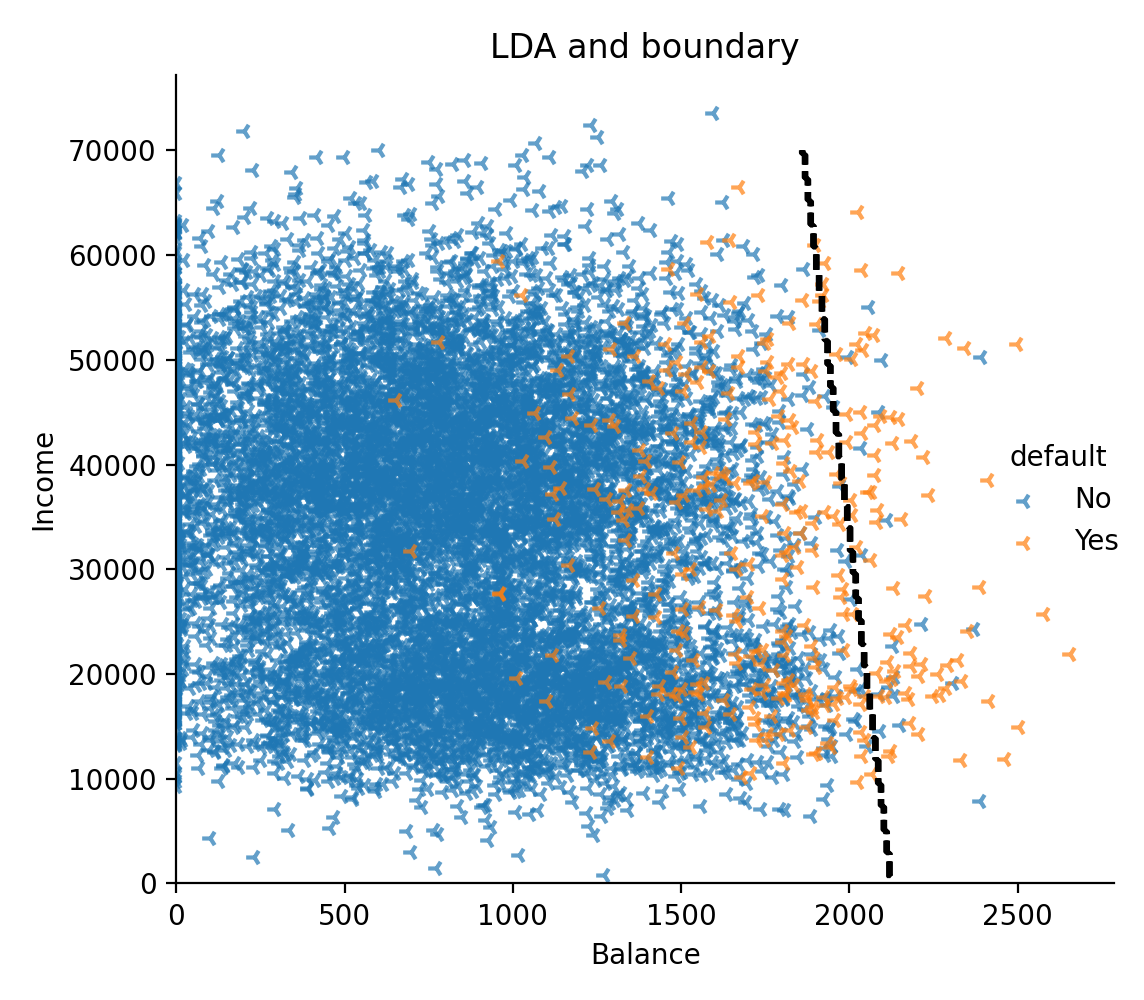
\includegraphics[width=.5\textwidth]{lda}
%   \end{minipage}
%   \begin{minipage}[p]{.2\linewidth}\hfill
%     \framebox(40,40){\Large KNN}
%   \end{minipage}
% \end{enumerate}

% \eject


% \bigskip

% \section*{Problem 2 \quad {\it Multiple choice  (5 points)}}
% Circle the roman numeral corresponding to the response that best fills in the blank or correctly answers  each of the following statements or questions.
% \begin{enumerate}[\bf (a)]
% \item The greater the degrees of freedom in a model, the greater the danger of \underline{\hspace{15ex}}.
%   \begin{enumerate}[\bf i.]
%   \item underfitting
%   \item overfitting
%   % \item extrapolation
%   \end{enumerate}

% \item Which of the following is a parametric classification approach?
%   \begin{enumerate}[\bf i.]
%   \item Random forests
%   \item K-nearest neighbors
%   \item Logistic generalized additive model
%   \end{enumerate}

% % \item Which of the three expected prediction error estimation methods reliably gives the lowest bias estimate?
% %   \begin{enumerate}[\bf i.]
% %   \item Validation set method
% %   \item $k$-fold cross-validation
% %   \item Leave-one-out cross-validation
% %   \end{enumerate}

% % \item Which of the three expected prediction error estimation methods  gives the highest variance estimate?
% %   \begin{enumerate}[\bf i.]
% %   \item Validation set method
% %   \item $k$-fold cross-validation
% %   \item Leave-one-out cross-validation
% %   \end{enumerate}
 
 
% % \item Which shrinkage method  \underline{\hspace{15ex}}.
% %   \begin{enumerate}[\bf i.]
% %   \item have a high bias
% %   \item have a high variance
% %   \end{enumerate}

% % \item Which subset selection method works best when the number of predictors $p$ is greater than the number of observations $n$?
% %   \begin{enumerate}[\bf i.]
% %   \item Best subset 
% %   \item Forward stepwise
% %   \item Backward stepwise
% %   \end{enumerate}

% \item Which of the two actions is more appropriate for increasing the recall of a binary classifier?
%   \begin{enumerate}[\bf i.]
%   \item Increase the threshold probability  of assignment to the positive class
%   \item Decrease the threshold probability  of assignment to the positive class
%   \end{enumerate}

% \item Which of the three expected prediction error estimation methods has the greatest variability?
%   \begin{enumerate}[\bf i.]
%   \item Validation set method
%   \item $k$-fold cross-validation
%   \item Leave-one-out cross-validation
%   \end{enumerate}

% \item In a 5-fold cross-validation, what proportion of the dataset is ultimately used in estimating the expected
%   prediction error?
%   \begin{enumerate}[\bf i.]
%   \item 5\%
%   \item 20\%
%   \item 50\%
%   \item 100\%
%   \end{enumerate}
% \end{enumerate}



\section*{Problem 2 \quad {\it Bayes' theorem (9 pts)}}
Given that $P (A) = 0.6$, $P (B) = 0.3$ and $P(C) = 0.1$ represent the production of machines in a
factory. The conditional probabilities of defective items are $P(D|A) = 0.02$, $P (D|B) = 0.03$ and
$P (D|C) = 0.04$.

\begin{enumerate}[\bf (a)]
\item Find the total probability $P(D)$. \pts{3}
 
  \item Find the \pts{3} probability that an item was produced by machine A, given that it is defective.
 
  \item Draw a Venn \pts{3} diagram depicting the interaction among the events $A$, $B$, $C$ and $D$ in sample space $S$.
    

\end{enumerate}

\section*{Problem 3\quad {\it Estimating a linear model (16 pts)}}
 
Given a vector of predictor variable samples $\bm{x}^{T} = \begin{bmatrix} 10 & 5 & 7 & 19 & 11 & 8\end{bmatrix}$
and corresponding response vector $\bm{y}^{T} = \begin{bmatrix}15 & 9 & 3 & 25 & 7 & 13 \end{bmatrix}$, the classical linear regression model can be written as
\begin{equation*}
  \hat{\bm y} = \bm X \hat{\bm w} 
\end{equation*}


\begin{enumerate}[\bf (a)]
 
\item Write the design matrix $\bm X$ in full assuming the model has an intercept (hint: the matrix should have two columns, the first being a column of 1's).  \pts{2} 

\item Using OLS (ordinary least squares) assumptions (see equation 4.59 on page 113 in \textbf{PMLI}), \pts{4} find $\bm{\hat w}$. (Show your work as much as possible, but the matrix multiplication can be done in Python/R/MATLAB. Include the code used if you are not submitting a Jupyter notebook.) 

\item Find the vector of predicted values  $\bm{\hat y}$. \pts{2}  
 
\item Find the vector of residuals $\bm e$. \pts{2}

\item Compute the mean squared error (MSE) of this model. \pts{2}

\item Compute the root mean squared error (RMSE) of the model. \pts{1}

\item Create a scatterplot of the data and show the least squares line \pts{3} in the plot.
  
\end{enumerate}


\section*{Problem 4 \quad {\it Logistic function (6 pts)}}
The logistic sigmoid function is given by:
\begin{equation}
  \bm\sigma(z) := \fr{1}{1 + e^{-z}}
\end{equation}

\begin{enumerate}[\bf(a)]
\item Produce a plot (in Python/R/Jupyter) of\pts{2} the function in the domain $z \in [-5,5]$.
\item Show that its derivative is given by: \pts{4}
  \begin{equation}
    \bm\sigma'(z)  = \fr{d\bm\sigma(z)}{dz} = [1 - \bm\sigma(z)]\bm\sigma(z)
  \end{equation}
\end{enumerate}

\eject
 \section*{Problem 5 \quad {\it Classifier performance (14 points) }}
An estimated classification model produces the following confusion matrix on a test set:

\begin{table}[h!]
  \centering \small
 % \caption{Confusion matrix (binary case)}
 % \label{tab:conf}
  \begin{tabular}{l l r r r}\toprule
    && \multicolumn{3}{c}{\it Predicted} \\
                                       &             & Class 0  & Class 1 & Total \\\midrule
    \multirow{2}{*}{\it Observed}& Class 0 & 9650 & 17 & ? \\
                                       & Class 1 &  265 & 68 & ? \\\midrule
    & Total & ? & ? & \\\bottomrule
  \end{tabular}
\end{table}
  
\begin{enumerate}[\bf (a)]

\item What is \pts{1} the number of false positives ($FP$)?

\item What is \pts{1} the number of false negatives ($FN$)?

\item What is \pts{1} the number of positive observations ($P$)?
  
\item What is \pts{1} the number of predicted positive  observations ($P^{*}$)?
  
\item Compute the test precision of the classifier. \pts{2} 
  
\item Compute the test recall of the classifier. \pts{2} 

\item Compute the test $F_1$-score of the classifier. \pts{2} 
\item Compute the test \pts{2}  accuracy of the classifier.
  
\end{enumerate}

\section*{Problem 6 \quad {\it Entropy (12 pts)}}
\textbf{PMLI} Exercise 6.3 (page 218).
  
\section*{Problem 7 \quad {\it Eigenvectors (6 pts)}}
\textbf{PMLI} Exercise 7.2 (page 266). Note: you can check your answer with Python/R/Matlab (include the code you used).

\section*{Problem 8 \quad {\it Linear system of equations (5 pts)}}
Reformulate the two equations:
\begin{align*}
  2x_{1} + 6x_{2} &= 8 \\
  5x_{1} + x_{2} &= 0 
\end{align*}
as a system of linear equations, and solve it for $[x_{1} \; x_{2}]^{T}$ using linear algebra.

\eject
\section*{Problem 9 \quad {\it Subgradients (7 pts)}}
\textbf{PMLI} Exercise 8.1 (page 314). [Context: the hinge loss is typically used as a loss function in classifier training, for example in support vector machines.]
\textbf{Important:} Answer the question along the following steps:
\begin{enumerate}[\bf (a)]
\item Sketch/plot the hinge loss function $f(x)$.\pts{2}
\item Write the piecewise subgradient/subderivative \pts{2} $\partial f(x)$ (see equation 8.14 on p.\ 276 for an example).
\item Evaluate the subgradient at the specified \pts{3} points in the exercise: $\partial f(0)$, $\partial f(1)$, $\partial f(2)$.
\end{enumerate}

% \section*{Problem 10 \quad {\it Optimization (9 pts)}}
% Implement an optimization algorithm of your choice to find  the value $\theta^*$ that maximizes the function
% \begin{equation*}
%   f(\theta) = \exp(-(\theta - 5)^{2}) + 0.1\sin(\theta -2)
% \end{equation*}
% in the interval $(0,12)$. Use any desired starting point. Show your code. Plot the function, indicating the optimal point obtained from your algorithm. State how many iterations you performed to obtain your result.
 


% \section*{Problem 5 \quad {\it Exploratory data analysis II (12 pts)}}
% The ultimate goal of this problem  is to apply linear regression techniques  to analyze \textbf{average vehicle ownership per household} in Massachusetts. However, in this problem set, you will only conduct exploratory data analysis.
% The data comes from the 2010 United States Census, which has been complemented with information from the American Community Survey (conducted between 2005 and 2010).
% The data, provided at a town level, includes:

% \begin{enumerate}
% \item Population Information
%   \begin{compactitem}
%   \item Race
%   \item Gender
%   \item Age
% \item Residence Type
% \item Language
% \item Employment
% \item Commuting Mode for Work
% \item Commuting Mean Travel Time
% \end{compactitem}

% \item  Household Information
% \begin{compactitem}
% \item Size
% \item Vehicle Ownership
% \item Income
% \end{compactitem}
% \end{enumerate}
% The data (\texttt{Massachusetts\_Census\_Data.xlsx}) covers all 351 towns/cities in Massachusetts. Import the 
% data into your notebook or workspace.
%   \begin{enumerate}[\bf(a)] 
%   \item Explore the data \pts{3} using either a matrix plot of the variables or scatter plots of the household vehicle ownership versus each of the variables (in a facet plot).
%   \item Plot the histograms of all the variables (organized neatly). \pts{3}
%   \item Generate a \pts{2} correlation matrix of all the variables. Identify which variables are highly correlated.
%   \item Determine if any of the \pts{4} variables should be transformed in any way to better predict or explain \textbf{average}
%     household vehicle ownership. Justify your solution by showing a scatterplot and correlation coefficient of the
%     transformed variable compared to its original form.  (\textit{Hint:} You may also have to manipulate the columns,
%     for instance: creating a column with percentage of households earning more than \$60,000 a year. Use your
%     exploratory plots to help here.)
    
%   \end{enumerate}
 

\end{document}

%%% Local Variables:
%%% mode: latex
%%% TeX-master: t
%%% End:
